\section{Evaluation}
\label{sec:evaluation}

We implement each algorithm from Section \ref{sec:algs} in the POX OpenFlow controller \cite{Pox} and run simulations using the Mininet 2.0.0 virtualization 
environment \cite{Lantz10}.  Simulations run on a Linux machine 
with four 2.33GHz Intel(R) Xeon(R) CPUs and 15GB of RAM.  Mininet is configured to run inside Oracle's VirtualBox \footnote{\url{https://www.virtualbox.org/}}
virtual machine and is allocated 4GB RAM and a single CPU.  
All generated virtual networks use Mininet's default software switch, Open vSwitch \footnote{\url{http://openvswitch.org/}}.  Unless otherwise noted, the \mdr 
controller algorithm runs inside the VirtualBox VM.


% Open vSwitch -- software switch, POX (OpenFlow controller), 

\subsection{Link Failure Detection Simulations}
\label{subsec:eval-pcount}

We run two sets of Mininet-based simulations to evaluate \pcnts. First, we measure the accuracy of \pcnt loss probability estimates and quantify how accuracy improves as more flows are monitored. 
Then, we consider how controller and switch processing time increases as \pcnt monitors more flows. 
%Unfortunately, switch processing time results are skewed because Mininet's software switch, Open vSwitch, 
%does not offer performance fidelity \cite{Lantz10}.  We comment further on this issue later in this section. 

%study the tradeoff between improving the accuracy of \pcnt packet loss estimates by monitoring more flows and the resulting increase in switch processing time 
%First, we study how the number of flows \pcnt monitors affects the accuracy of its packet loss estimates. Then, detection time is quantified as a function of the number of monitored flows.  
%Our simulations configure \pcnt such that all measurement windows are non-overlapping.  
%This means that for each window, $w$, \pcnt accounts for every dropped packet of a monitored flow, 
%meaning that the accuracy of \pcnt loss estimates are determined by its window size ($w$) and the number of monitored link flows ($k$).

%We can modify \pcnts's window size ($w$) and number of monitored link flows ($k$) to control the number of packets \pcnt uses to estimate the loss rate.  
%In this simulation, we evaluate 
%hus, the accuracy of \pcnt loss rate estimates are a function of the number of packets considered in a sampling window $w$. 

%{\bf Setup.}
{\bf Accuracy of Loss Probability Estimates.}
For the dumbbell topology shown in Figure \ref{fig:eval-pcount-setup}, we use \pcnt to measure the packet loss over link $(u,d)$.  We generate $m$ multicast groups
where each $h_1,h_2, ..., h_m$ multicasts packets to terminal nodes $s_1, s_2, ..., s_m$ at a constant rate of $60$ packets per second, the standard sampling rate of PMUs.  \base is used
to implement multicast, resulting in $m$ separate flow table entries at $u$ and $d$.  At the end of the section we comment how our results apply to \merges. We let $m=\{10,20,30,40,50\}$
\footnote{Simulations run prohibitively slow for $m>50$ due to CPU overload.} %the CPU overhead of each of the $m$ constant bit rate flows made each simulation run prohibitively slow.}
and, using Mininet, drop packet traversing $(u,d)$ using a Bernoulli process with loss probability $p=\{.01,.05,.10\}$.  
%Let $w$ be \pcnt loss estimates are a function of its window size ($w$) and number of monitored link flows ($k$).

%In this simulation, we measure how close \pcnt loss probability estimates are to $p$ for different $w$ and number of monitored flows ($k$).
In this simulation, we quantify how the accuracy of \pcnt loss estimates -- measured relative to the true underlying loss rate, $p$ -- as we modify the number of flows \pcnt monitors. 
Recall from Section \ref{subsec:pcnt} that \pcnt accounts for every dropped packet of a flow it monitors, meaning that the only error in \pcnt estimates results from unmonitored flows.
%Here we quantify how the accuracy of \pcnt loss estimates change as we modify the number of flows \pcnt monitors.  
Because the same trends hold across all $m$ and $p$ values, we describe a single representative case, where $m=10$ and $p=.05$, below.
%We find the same trends hold across all $m$ and $p$ values.  A representative case, where $m=10$ and $p=.05$, is described below.

%This means that for each window, $w$, \pcnt accounts for every dropped packet of a monitored flow, 
%meaning that the accuracy of \pcnt loss estimates are determined by its window size ($w$) and the number of monitored link flows ($k$).

Figure \ref{fig:pcount-loss-windows} compares the $95\%$ confidence intervals of \pcnts's link loss probability estimates -- centered around the true loss probability ($.05$) for consistency -- 
as a function of window size $w =\{0.5,1,...,5\}$ seconds. \pcnt is configured such that each measurement window starts only after the packet loss from the previous window has been computed.
Results are shown where \pcnt monitors $k=\{10\%,40\%,70\%,100\%\}$ of $(u,d)$ flows (each monitored flow is selected randomly).  The confidence intervals for each $w,k$ pair are computed
over $100$ simulation runs.

% in which each monitored flow is selected randomly. 
%For consistency, the $95\%$ confidence interval curves are centered around the true loss probability ($.05$). 

\pcnt loss rate estimates are extremely accurate: the $95\%$ confidence interval, across all $w$ and $k$, lies within $15\%$ of the true loss probability.  This is the case even when \pcnts's 
estimate is based on only $30$ packets (occurs when $k=10\%$ and $w=0.5$).  Figure \ref{fig:pcount-loss-pkts}, which plots link loss probability estimates as a function of the number of 
packets considered during each simulation run, shows that after \pcnt considers $75$ packets its mean loss probability estimate is within $2\%$ of the true loss probability.  
\footnote{This accuracy is not surprising since loss probability estimate is averaged over $100$ simulation runs.}
As expected, \pcnt accuracy increases with larger $k$.  For each $k$, the standard deviation (of \pcnt loss probability estimates) decreases as a function of the square root of $w$.  
%However, since \pcnt loss rate estimates are 

%Figure \ref{fig:pcount-loss-pkts} plots link loss probability estimates as a function of the number of packets considered during each simulation run.  
%After \pcnt considers $75$ packets its mean loss probability estimate is within $2\%$ of the true loss probability.  This accuracy is not surprising since loss probability estimate is 
%averaged over $100$ simulation runs. 


%Since \pcnts's aim is to estimate loss probabilities over a single window, a more telling statistic is the standard deviation. Figure \ref{fig:pcount-loss-windows} 
%shows that the standard deviation, for each $k$, decreases as a function of the square root of $w$.  The same trend holds when we %consolidate the four curves from Figure \ref{fig:pcount-loss-windows}
%plot the same link loss probability estimates as a function of the number of packets, rather than window size, \pcnt considers over each simulation run (Figure \ref{fig:pcount-loss-pkts}).
%We find that after \pcnt considers approximately $750$ packets, the confidence intervals lie within $20\%$ of the true probabilities, suggesting that individual \pcnt loss probability
%estimates are extremely accurate.   %Accuracte loss estimates were expected because 


{\bf Processing Time.}
%Next we quantify the processing time at the network switches in handling \pcnt statistic queries. [mention this is the primary time] 
%Next, we quantify switch processing time associated with handling \pcnt statistic queries. 
Next, we quantify how \pcnt processing time increases when \pcnt monitors additional flows.  We measures packet loss over $(u,d)$ from Figure \ref{fig:eval-pcount-setup}.
Processing time is measured as the time between when \pcnt sends its first statistic query and when \pcnt computes its packet loss estimate. Recall from Section \ref{subsec:pcnt} 
that if \pcnt monitors packet loss of $k$ flows traversing $(u,d)$, \pcnt sends $k$ statistic queries to $u$ and one aggregate query to $d$. 

\pcnt is configured such that each measurement window starts only after the packet loss from the previous window has been computed. Additionally, \pcnt window size is fixed to $2$ and 
the loss threshold is set to $0$.
Because Mininet multiplexes CPU resources using the default Linux scheduler, we found that running the constant rate PMU flows introduces unwanted CPU contention, adding noise to 
our results.  For this reason, we create only a single multicast group (with source $h_1$ and a single sink $s_1$) 
but do not actually send any packets between the two hosts. To further reduce CPU contention, we run \pcnt as a remote control application, outside of the VirtualBox VM.

As computed, processing time accounts for (a) the time at the controller
to generate $k+1$ statistic queries, (b) the transmission delay associated with sending the $k+1$ statistic queries from the controller to $u$ and $d$, 
(c) the network delay in sending each statistic query from the controller to switch, (d) total time to process the statistic query at $u$ and $d$, (e) the delay in sending the $k+1$ query results
from switch to controller, and (f) the latency in receiving and recording statistic query replies at the controller. % and computing packet loss at the controller. 
We subtract (c) and (e), the network delay between controller and switches, from the measured processing times.  Because the combined delay of (a), (b), and (f) accounts for less
than $1\%$ of the overall processing time, part (d), the time to process statistic queries at $u$ and $d$, determines the overall processing times.



%Recall from Section \ref{subsec:pcnt} that if \pcnt monitors packet loss of $k$ flows traversing $(u,d)$, \pcnt sends $k$ statistic queries to $u$ and one aggregate query to $d$. 
%We measure detection time as the time between when \pcnt sends its first statistic query and when \pcnt computes its packet loss estimate.  This time window accounts for (a) the time at the controller
%to generate $k+1$ statistic queries, (b) the transmission delay associated with sending the $k+1$ statistic queries from the controller to $u$ and $d$, 
%(c) the network delay for each statistic query to reach the appropriate switch, (d) total time to process the statistic query at $u$ and $d$, (e) the delay in send the $k+1$ query results
%from switch to controller, and (f) the latency in receiving and recording statistic query replies. % and computing packet loss at the controller. 

%\footnote{We did additionally measure the time to generate and send OpenFlow statistic queries from the controller, along with time to process and record query results at the controller. 
%This controller processing time is insignificant when compared to switch processing time: at most total controller processing time is $150$ times smaller than the total switch processing time. }
%Using the topology from Figure \ref{fig:eval-pcount-setup}, we monitor packet loss over $(u,d)$. \pcnt is configured such that each measurement window starts only after the packet loss from
%the previous window has been computed. Additionally, \pcnt window size is fixed to $2$.  

%Recall from Section \ref{subsec:pcnt} that if \pcnt monitors packet loss of $k$ flows traversing $(u,d)$, \pcnt sends $k$ statistic queries to $u$ and one aggregate query to $d$.  
%We measure the total switch processing time as the time between when \pcnt sends its first and last statistic query, minus the average controller-to-switch delay.  

Figure \ref{fig:pcount-dtime} shows the processing time, computed as described in the previous paragraph, as a function of the number of flows \pcnt monitors, $k$.
\footnote{Fake multicast groups and corresponding flow table entries are generated and installed at $u$ and $d$ in cases where \pcnt monitors more than the $1$ multicast group.}
Each data point is the mean computed over $50$ simulation runs. To measure the effect of flow table size on query processing time, we install $r$ additional flow table entries at $u$ and $d$.

We find that processing time increases quadratically with $k$ and there is a significant gap in processing time between each $r$.  In practice, we expect non-empty flow tables so the $r=0$ curve
is overly optimistic.  Therefore, to reasonably achieve sub-second processing time, our results show that fewer than $75$ flows can be monitored. 

Because the switches are completely idle during each simulation run, except for the time to process the read state queries, and the software switches used have
considerably more powerful CPUs relative to hardware switches \cite{Curtis11,Rotsos12}, these results likely underestimate processing time.  
Nonetheless, these results underscore the high cost in monitoring a large number of flows. 
%We expect the query processing 

%Due to Mininet's lack of performance fidelity, each statistic query takes $O(r+k)$ time to process rather than $O(1)$ time (provided by real hardware switches) \cite{Lantz10}. As a result,
%processing time increases quadratically with $k$ and there is a significant gap in processing time between each $r$.  If real hardware switches were used, we would expect
%processing time to increase linearly as $k$ grows and that the four separate $r$ curves from Figure \ref{fig:pcount-dtime} would collapse into one single curve.

{\bf Summary.}
%Although the processing time results are skewed in favor of \pcnts, the slow processing times associated with monitoring large numbers of flows and the highly accurate loss estimates
The slow processing times associated with monitoring large numbers of flows and the highly accurate loss estimates for even small $k$ strongly suggest that $k$ should be small.
Because the software switch skews the processing time results in favor of \pcnts, we expect that even a stronger case for using small $k$ can be made using hardware switches.
However, we caution that the (Bernoulli) loss process is biased in favor of \pcnt because we found loss rates to be nearly uniform across all flows traversing $(u,d)$.

%that a trade-off between accuracy and processing time exists when determining
%negatively by a factor of $r+k$, the results underscore that a trade-off between accuracy and processing time exists when determining
%how many flows to monitor with \pcnts. Fortunately, we found \pcnt loss estimates to be highly accurate even when monitoring a small percentage of flows ($10\%$) traversing $(u,d)$, suggesting
%that small $k$ should suffice.  As further evidence, we observed a small marginal increase in accuracy along with a significant penalty (in terms of detection time) resulting from using 
%large $k$.  However, we caution that the (Bernoulli) loss process is biased in favor of \pcnt because we found loss rates to be nearly uniform across all flows traversing $(u,d)$.

%In Section \ref{subsec:merge}, we stated that \merge can speed \pcnt processing because, with \merges, \pcnt can install and query fewer flow table entries to achieve similar accuracy results
%when monitoring more \base flows.
%reduce switch processing time by reducing the number of \pcnt statistic queries since multiple flows may be using the same forwarding rule. 
%Our results suggest that the savings in processing time can be significant. 

%The trade-off between accruacy and processing time suggests that \merge can improve \pcnt results.  As detailed in Section \ref{subsec:merge}, \merge can reduce the 

%In summary, determining how many flows to monitor involves a trade-off between accuracy and processing time.Although processing times from our simulations are skewed negatively by a factor of $r+k$, the results underscore the significant penalty (in terms of detection time) in monitoring a large number of flows. 
%Fortunately, we find \pcnt loss estimates to be highly accurate even when monitoring a small percentage of flows ($10\%$) traversing $(u,d)$.  This allows for fast and accurate packet loss detection.%Further, the impressive accuracy of \pcnt results when monitoring a small percentage ($10\%$) of flows suggest that only a fraction of flows need to be monitored. 

%Our findings also confirm that our conjecture in Section \ref{subsec:merge} that \merge can improve \pcnt results.  Recall that \merge replaces individual forwarding rules (when possible) that 
%have the same set of
%outports with a single flow table entry. As a result, when \pcnt copies the flow table entry, $e_i$, of a monitored flow, $f_i$, for tagging and counting purposes, \pcnt indirectly monitors all other 
%flows using $e_i$ (as a result of \merges).  This allows \pcnt to derive the accuracy gains of monitoring multiple flows (each flow using $e_i$) but at the cost of monitoring a single flow 
%(only a single \pcnt statistic query must be sent to $u$, rather than one query per flow using $e_i$). 
%to estimate loss over a sample of more than $60$ packets/second, thereby boosting accuracy, yet only a single \pcnt statistic query must be sent to $u$ (rather than one query per flow using $e_i$

%when \pcnt monitors a flow, $f_i$, $f_i$ may map to a rule, $e_i$, used by multiple flows.  By tagging and counting all packets matching $e_i$, \pcnt estimates loss over a sample
%of more than $60$ packets/second, thereby boosting accuracy, yet only a single \pcnt statistic query must be sent to $u$ (rather than one query per flow using $e_i$).

%{\it [TODO]: mention \merge is beneficial because fewer queries.  this is the case whether query processing time is linear or constant}
%
%{\it [TODO]: In summary, determining how many flows to monitor involves a trade-off between accuracy and processing time.  Although processing times are skewed by a factor of $r+k$, 
%the results underscore the significant time penalty (in terms of detection time) in monitoring a large number of flows.  Further, the impressive accuracy of \pcnt results even when 
%a small percentage ($10\%$) of flows are monitored suggest that only a fraction of flows need to be monitored. } 


%\begin{figure*}[t]
%  \begin{center}
%  	\subfigure[Dumbbell topology used in the \pcnt evaluation.]{ \label{fig:pcount-res}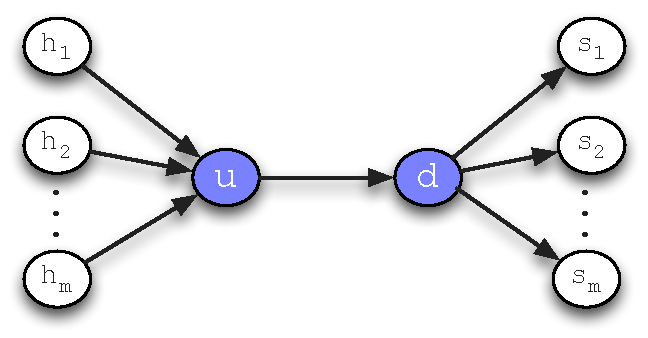
\includegraphics[scale=0.51]{figs/pcount-setup.pdf}}
%    \subfigure[Loss estimates as function of \pcnt window size.]{\label{fig:pcount-loss-windows}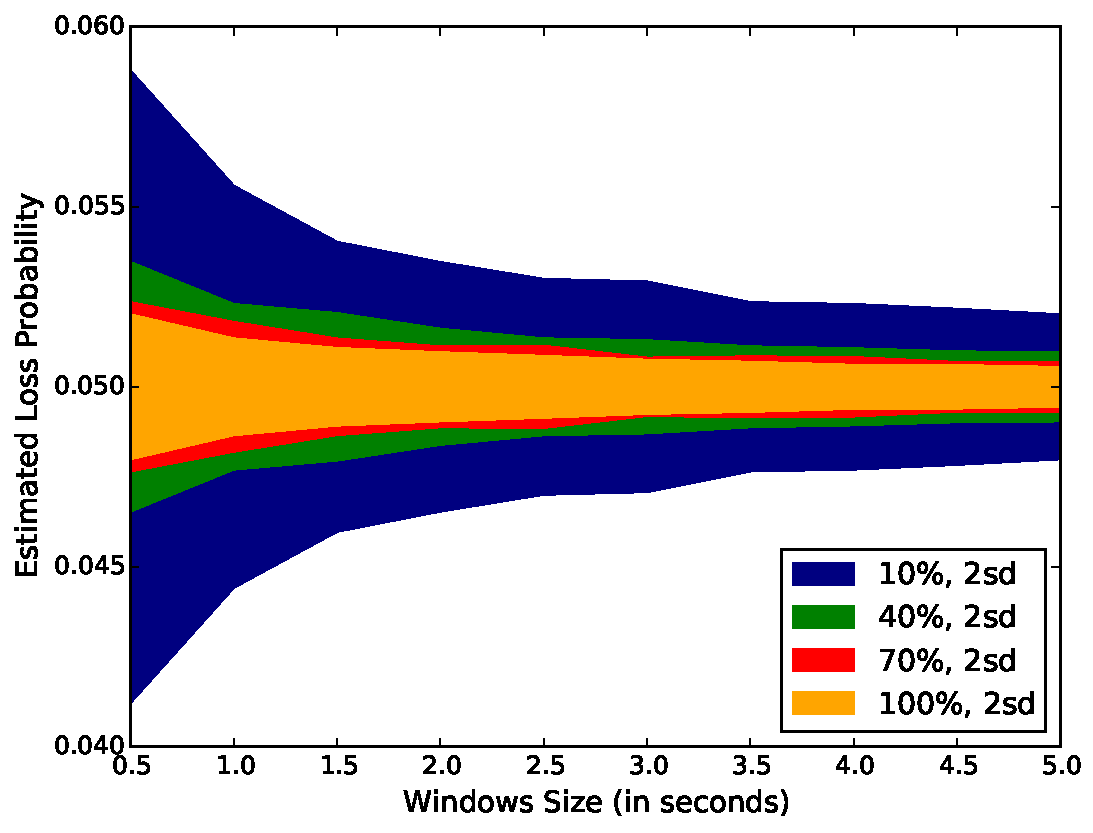
\includegraphics[scale=.33]{figs/pcount-loss-windows.pdf}}
%    \subfigure[Loss estimates as function of number of packets.]{\label{fig:pcount-loss-pkts}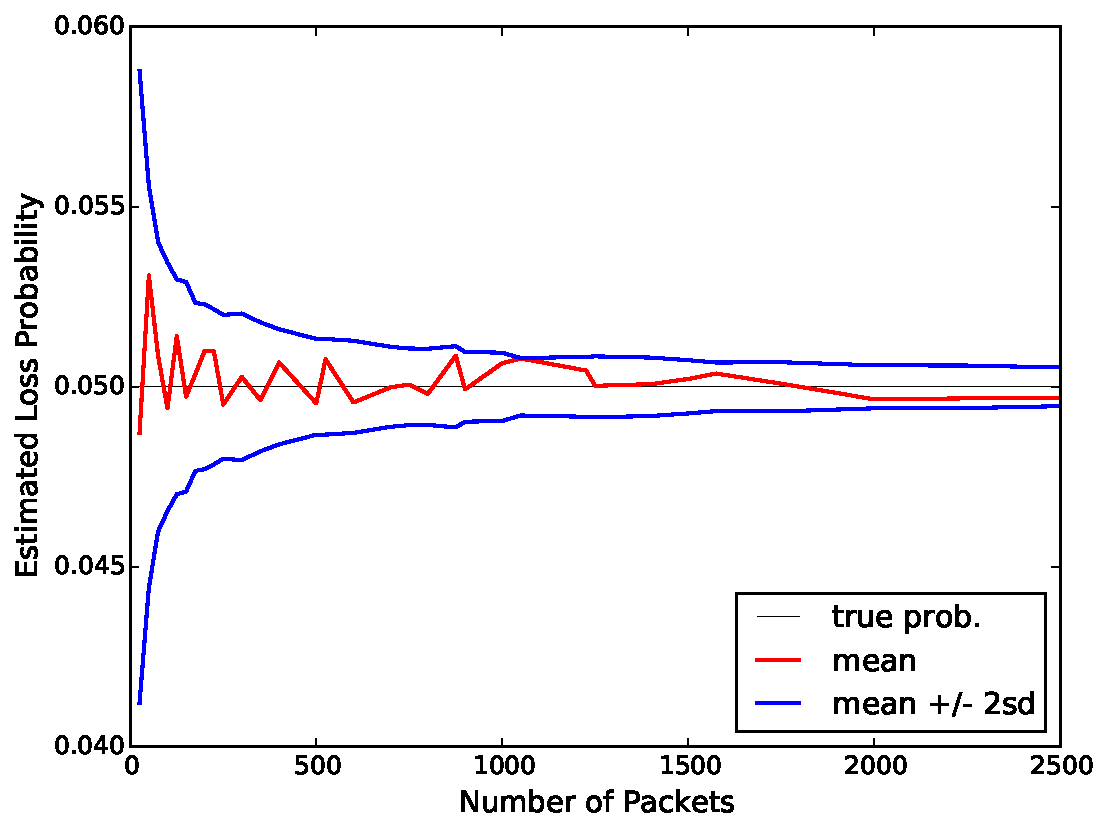
\includegraphics[scale=0.33]{figs/pcount-loss-pkts.pdf}}
%  \end{center}
%	\caption{Accuracy of \pcnt loss probability estimates over a single link, $(u,d)$, from Figure \ref{fig:eval:pcount-setup}.}
%  \label{fig:pcount-res}
%\end{figure*}


\begin{figure}
  \centering
   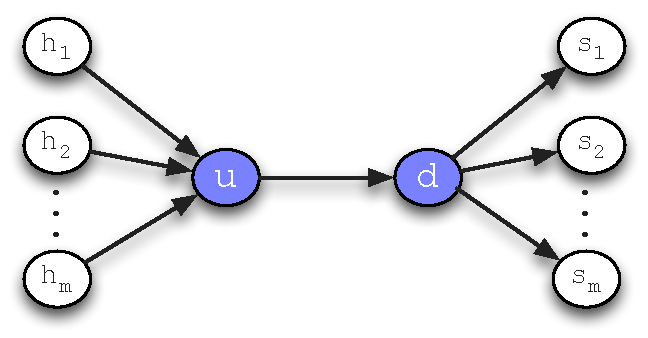
\includegraphics[scale=0.75]{figs/pcount-setup.pdf}
\caption{Dumbbell topology used in the \pcnt evaluation.}
\label{fig:eval-pcount-setup}
\end{figure}

\begin{figure*}[t]
  \begin{center}
    \subfigure[Loss estimates as function of \pcnt window size.]{\label{fig:pcount-loss-windows}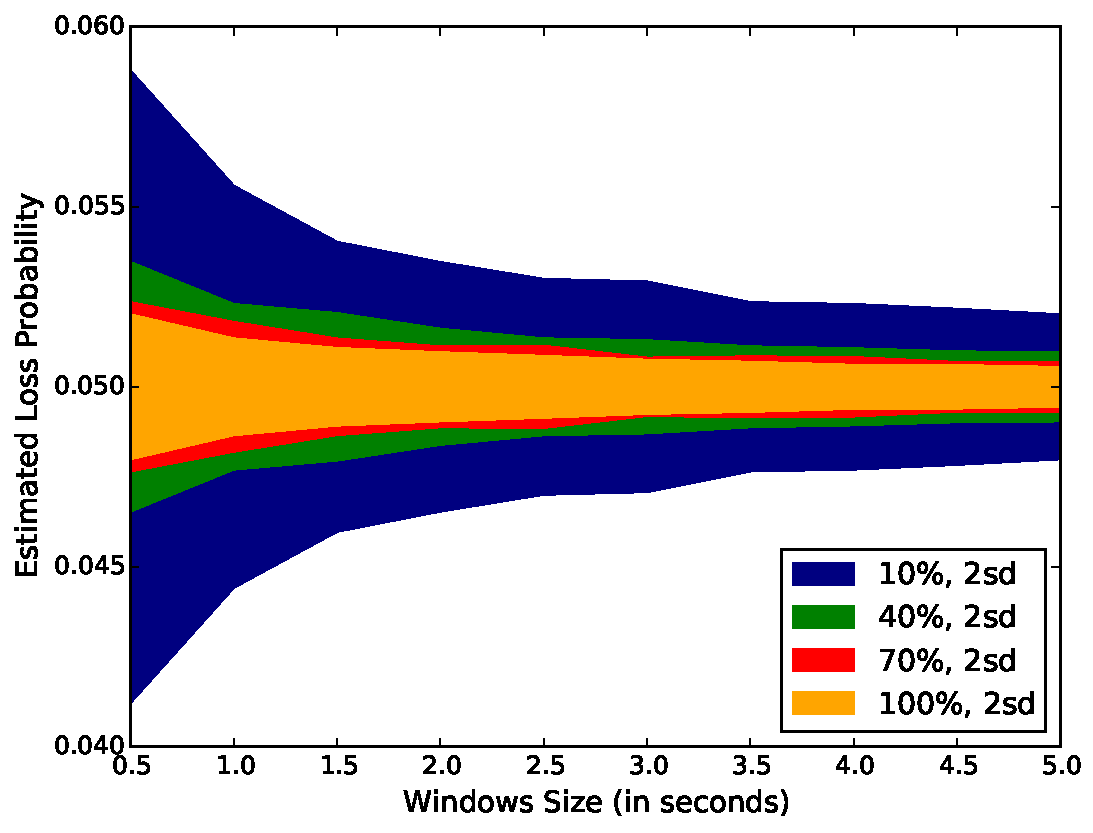
\includegraphics[scale=0.4]{figs/pcount-loss-windows.pdf}}
    \subfigure[Loss estimates as function of number of packets.]{\label{fig:pcount-loss-pkts}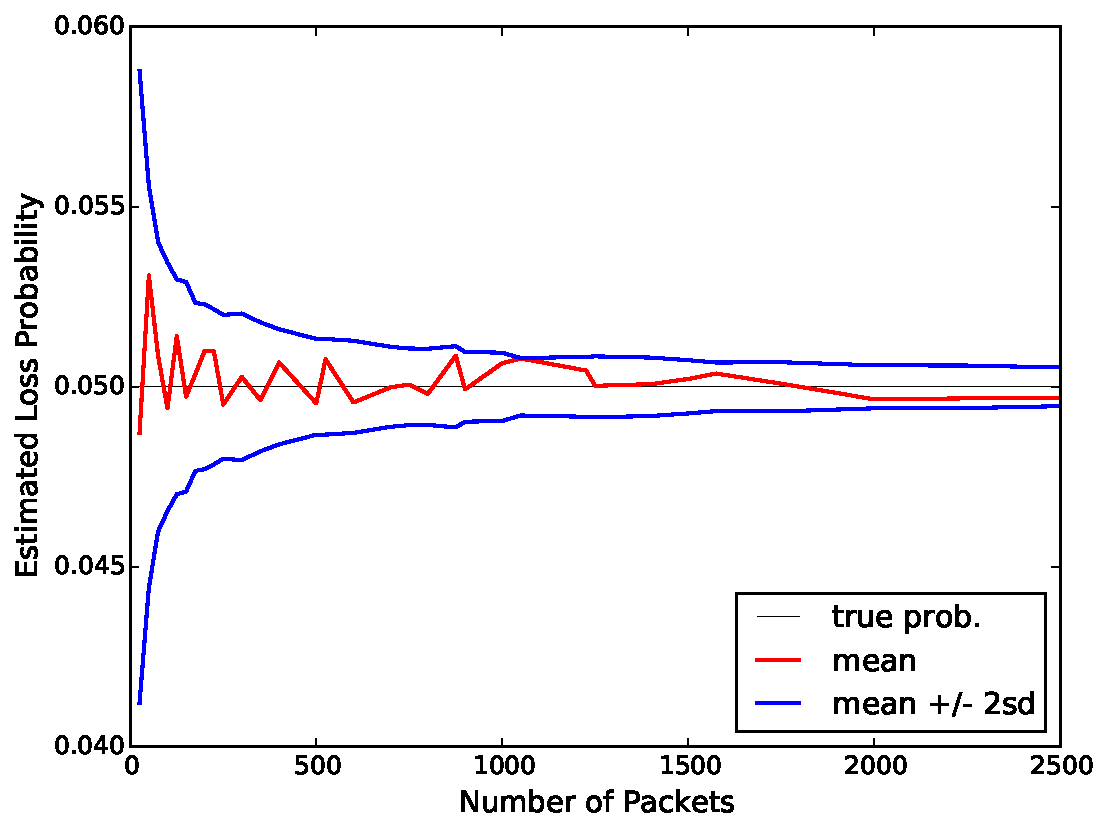
\includegraphics[scale=0.4]{figs/pcount-loss-pkts.pdf}}
    \subfigure[Processing time, with $95\%$ confidence intervals, as a function of number of monitored flows.]{\label{fig:pcount-dtime}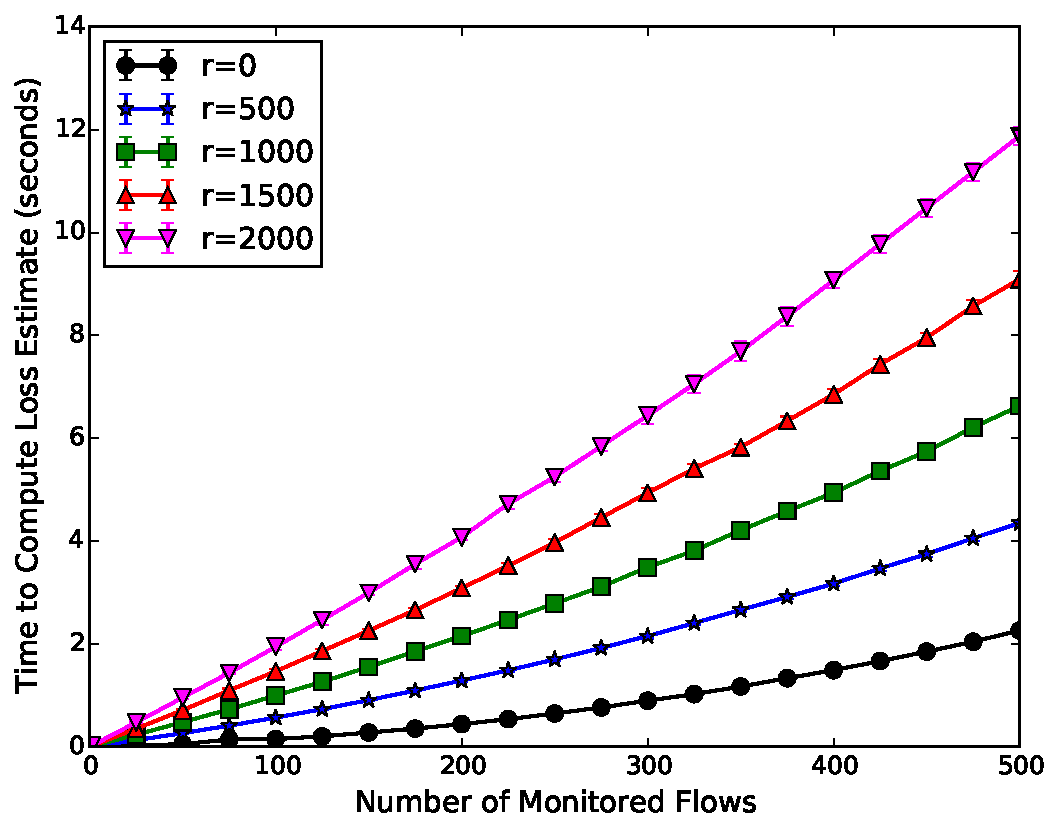
\includegraphics[scale=0.4]{figs/pcount-dtime-w5-j4000.pdf}}
  \end{center}
	\caption{\pcnt results monitoring a single link, $(u,d)$, from Figure \ref{fig:eval-pcount-setup}.}
  \label{fig:pcount-res}
\end{figure*}



\subsection{Backup Tree Installation Simulations}
\label{subsec:eval-backuptrees}

In this section, we simulate the failure of a single link and then measure recovery time, control plane signaling, and garbage collection overhead for \pre and \post both with and without
the \merge optimization. We aim to answer the following questions with these simulations: 
\begin{itemize}
	\item How effective is \steiner in reusing primary tree edges and in providing opportunities for backup tree installation algorithms to reuse primary tree forwarding rules?
	\item How much faster does \pre recover from link failure than \posts? 
	\item How many fewer control messages are needed to install backup trees under \pre versus \posts?
	\item How much control state does \pre pre-install?
	\item In terms of recovery time, control plane signaling, and garbage collection, how much does \merge improve performance relative to \bases?
\end{itemize}
%We use simulations to quantify \pres's faster recovery time relative to \post and \merges's benefits versus \bases: faster recovery time when using \posts, less preinstalled state  under \posts, and reduced garbage collection.  


% Changes to plots: (a)  should label lower bound with algorithm name (e.g., Reactive)

{\bf Setup.}
We use IEEE bus systems $14$, $30$, $57$, and $118$ \footnote{\url{http://www.ee.washington.edu/research/pstca/.}}
and synthetic graphs based on these IEEE bus systems to evaluate our algorithms.  Each bus system consists of buses -- electric substations,
power generation centers, or aggregation points of electrical loads -- and transmission lines connecting those buses. The IEEE bus systems are actual portions of the North American
 transmission network, where PMUs are being deployed.  Note that the bus system number indicates the number of buses (nodes) in the graph (e.g., bus system $57$ has $57$ nodes).  
Synthetic graphs are generated using a procedure described in one of our previous papers \cite{Gyllstrom12} that uses an IEEE bus system as a template to generate
graphs with the same degree distribution as the template bus system.  

We assume that the communication network mirrors the physical bus system topology. It is assumed that
an OpenFlow switch is co-located at each bus and that two unidirectional communication links, one in each direction,
connects these switches following the same configuration as the bus system's transmission lines.  Additionally, we connect each switch with a leaf host using a bidirectional communication link.  
%As a result, each communication network used in our simulations has the same number of hosts and switches.
In this setup, the PMUs measure voltage and current phasors at the buses, then these measurements are sent by the bus's attached host to its first-hop switch, and lastly 
the first-hop switch multicasts the PMU measurements using the network of OpenFlow switches to a set subscribing hosts (terminals).  

For each bus system $n$, we generate synthetic topologies with $n$ switches, $n$ hosts, and set all link weights to $1$.  Then, we randomly create $m=\{1,2,...,\frac{n}{2}\}$ multicast groups, 
each with $n/3$ random terminal hosts, and use the \arbor approximation proposed by Charikar et al. \cite{Charikar98} to compute the $m$ primary trees. \steiners, with $\alpha=1.1$, is then used
to pre-compute, for each primary tree, a backup tree for each primary tree link.
Next, a random communication link, $l$, that is used by at least one primary tree is chosen to fail (i.e., drop enough packets to trigger a \pcnt alert), 
triggering the installation of backup trees using either \post or \pres.  For each $m$, we generate $35$ different synthetic graphs and $3$ random sets of multicast groups, 
yielding a total of $105$ simulation runs per $m$.  
%Primary trees are computed using the \arbor approximation proposed by Charikar et al. \cite{Charikar98} and backup trees computed by \steiner with $\alpha=1.1$. 

The results described in the remainder of this section are those from synthetic topologies generated using IEEE bus system $57$ as a template. The trends are consistent across 
all other networks. Switches in the networks generated using IEEE bus system $57$ have an average diameter of $11.75$ and average degree $3.74$.   
%The $35$ synthetic graphs based on bus system $57$ graphs have an average diameter of $11.75$ and average degree $3.74$. 
For each of the $m$ multicast groups, we initially attempted to multicast packets at a constant rate flow of $60$ packets per second from the root host but this 
caused CPU overload.  Instead, in each simulation run we only initiated the constant rate flows for the primary trees using the failed link.

%{\it Missing the following parameters: link weights are $1$, $\alpha$ for SA computation, what is pcount loss threshold?, how are we inducing loss at links?}


\subsubsection{\steinern Results}
\label{subsubsec:tree-stats}

% assume e2e delay 5ms & 8ms 
The primary trees computed using the \arbor approximation described in Section \ref{subsubsec:steiner-approx} have an average root-to-terminal hop count of $7.54$, while the \steiner backup trees are 
slightly larger with an average end-to-end (E2E) length of $8.4$.  Based on the E2E latency requirements reported in Section \ref{subsec:pmu-requirements}, the 
per-link delay in our simulated topologies would need to be in the range of $0.6-1$ms to satisfy QoS requirements using these multicast trees.  
\footnote{The average root-to-terminal path lengths were largest for IEEE bus system $57$ and the synthetic graphs based on this bus system.  The multicast trees computed for bus system $118$ 
have an average E2E path length approximately $1$ hop fewer than those for bus system $57$, even though IEEE bus system 118 has more than twice as many nodes as bus system $57$.  This is mainly 
due to bus system $118$'s higher density (than bus system $57$). }
%Mainly because bus system $118$ is more dense, its average degree is $4.04$.}
%These latencies are certainly attainable within the portions of the power


%Although IEEE bus system 118 has more than twice as many nodes as bus system $57$, the primary and backup trees computed over bus system $118$ are smaller than those computed
%using bus system $57$.  E2E is a larger graph than  the average E2E path length is  
%This implies that the total per-hop delay must be in the range of $0.6 - 1 $ms to meet the most challenging PMU application E2E latency requirements (Section \ref{subsec:pmu-requirements}).  

On average, the \steiner backup trees have stretch of $1.17$. %, a common goodness measure for multicast trees, of $1.17$.  
Stretch is defined per multicast tree and is the ratio of path length from the root to terminal along the multicast tree to the length of the direct unicast path. 
For comparison with \steiner results, we compute a second backup tree for each primary tree, $T_i^l$, 
by running the \arbor approximation described in Section \ref{subsubsec:steiner-approx} over the original graph with $l$ removed. We denote the set backup trees for $l$ computed using this algorithm
as $B^l$. 
%As expected, the $B^l$ backup trees are smaller than the $\hat{T}^l$ backup trees ($w(\hat{T}^l)/w(B^l) = 1.08$) because $B^l$ trees are computed independent of the primary tree while $\hat{T}^l$

The $B^l$ backup trees are marginally smaller than the $\hat{T}^l$ backup trees: $w(\hat{T}^l)/w(B^l) = 1.08$.  This is expected because $\hat{T}^l$ is computed using 
a heuristic to guide \steiner to reuse primary tree edges, while $B^l$ trees are an approximation of the least cost directed tree (and so are computed independent of the edges used by the primary tree). 

However, $\hat{T}^l$ reuses more primary tree edges ($\hat{T}^l$ reuses $59\%$ of primary tree edges versus $41\%$ under $B^l$). Most importantly, when comparing $\hat{T}^l$ and $B^l$ with 
the primary tree, $\hat{T}^l$ has more common nodes with the primary tree that have the same children in $\hat{T}^l$ and the primary tree ($55\%$ of $\hat{T}^l$ nodes) 
than $B^l$ ($38\%$ of $B^l$ nodes).  
%primary tree and share the same children as its primary tree at $55\%$ of $\hat{T}^l$'s nodes instead of $38\%$ with $B^l$ forwarding rules ($55\%$ instead of $38\%$ with $B^l$).  
This last point is important because this allows $\hat{T}^l$ to reuse more primary tree rules once $\hat{T}^l$ is installed.
In summary, these results suggest that \steiner computes backup trees only slightly larger than an approximation of the least cost tree with a significant gain in primary tree 
edge and forwarding rule reuse. 

%Recall from Section \ref{subsec:steiner} that \steiner first attempts to compute a backup tree, $\hat{T}_i^l$, using a graph copy where 
%the links weights of $\hat{T}_i^l$'s associated primary tree are set to $0$.  If the cost of the resulting backup tree, $\hat{B}_1$, is sufficiently small, $\hat{T}_i^l = \hat{B}_1$ is returned. 
%Otherwise, the minimum cost backup tree, over the original graph without the failed link, is computed and returned.  We denote this second tree as $\hat{B}_2$   In almost all cases $\hat{B}_1$ satisifize
%the cost constraint; on average, $w(\hat{B}_1)/w(\hat{B}_2) = 1.08$.  This modest increase in tree size %link weights of $T_i$

%Graph properties: mean graph diameter=$11.75$, average degree = $3.74$
%Backup Tree properties: avg BT e2E = $8.64$, stretch = $1.17$, $w(BT_1)/w(BT_2) = 1.08$, $c(BT_1)/c(BT_2) = 0.67$, mean percentage PT nodes reused = $78\%$ vs $65\%$, mean percentage PT edges reused = $59\%$ vs $41\%$.

% Graph properties -- degree and diamter (with and without failed link)
% Feasability of E2E latency requirements -- reasonable tree yields PT hop count of x, meaning the avg link delay must be < ?
% Bunchy vs straw man results
% open questions: PT vs BT size, 


%{\bf Signaling Overhead.}
\subsubsection{Signaling Overhead}
\label{subsubsec:eval-signaling}

Next, we compare the number of control messages required to install backup trees as function of the number of primary trees ($m$) installed in the network.  Figure \ref{fig:msgs57} shows the results for 
\post running in \base and \merge mode, referred to as \posts+\base and \posts+\merges, respectively; a lower bound for \post (\posts+\lbs); and \pre in \base mode, denoted as \pres+\bases.  
Note that the results for \pre are the same using \base and \merge because \pre requires 
that only the root node of each backup tree needs to be signaled to activate the backup.  We shall later see how \base and \merge affect the number of forwarding
rules \pre pre-installs.

\posts+\lb computes the lower bound at each switch, $v$, used by a backup tree for the failed link ($l$) and returns the sum of each node's lower bound.
At $v$, the lower bound computation first finds the set of outports used by all primary and backup trees and then eliminates any backup tree with the same outports as a primary tree
(these backup trees can reuse the primary tree forwarding rule rather than installing a new one).  
Among the remaining backup trees, the number of unique sets of outports, $b$, is equal to the minimum number of 
forwarding rules that must be installed at $v$: if fewer than $b$ rules are installed at $v$, packets corresponding to at least one multicast group would not match with a rule that forwards
packets out the correct set of ports.
%Because at least a single flow table entry is needed for each unique set of outports to ensure correct forwarding, the optimal solution cannot be less than the lower bound. 

As expected, we find that \pre requires less signaling overhead than \posts, including even \posts+\lbs.   \pre activates the backup trees by sending a control message
(to install a pre-computed forwarding rule) to the root switch of each of backup tree using the failed link, whereas \post must signal multiple switches to install each 
backup tree. %The mean for $m_l$ starts at $1$ (when $m=1$) and increases linearly as function of $m$ to a maximum of $6.5$ (for $m=28$).  
%(for each backup tree, \post signals each switch with a pre-installed flow under \pres). 

%Likewise, the number of control messages for \bases, \merges, and the lower bound all increase linearly with $m$.  

%{\it TODO: mention that the savings for between $2$ and $2.5$ for $m \geq 15$.}
For \posts, the gap between \base and \merge increases as we introduce more primary trees.  
When $m=1$ there are no opportunities for \merge to consolidate forwarding rules so \merge and \base require exactly 
the same number of control messages to install the backup tree.

As $m$ grows, three factors contribute to an increasing gap between \base and \merges.  One, there are more primary tree forwarding rules 
(installed in the network) that \merge can reuse. Our results show that for $m \geq 7$, $75\%$ of \merge savings (versus \bases) are due to reusing primary tree forwarding rules. Two, 
as $m$ increases more graph edges are used: when $m=28$, $90\%$ of all network links are used by at least one primary tree and is at least $80\%$ for $m \geq10$. 
This benefits \merge because it increases the likelihood that at any switch a backup tree shares the same outgoing links as at least one primary tree. 
%This near network-wide use of graph edges is favorable for \merge because it increases the likelihood that at any switch a backup tree shares the same outgoing links as at least one primary tree. 
Three, as $m$ increases more primary trees are affected by a link failure causing more backup trees to be installed for each link failure. 
This provides additional opportunities for \merge to consolidate flow table entries with other backup trees.
%Three, as $m$ increases more backup trees are installed after a link failure since more primary tree are likely to use $l$. This provides additional opportunities for \merge to consolidate 
%flows with other backup trees. %with common forwarding. 
However, this third factor is less significant than the previous two, as only $25\%$ of \merge savings are due to consolidating flows with other backup trees.
%Overall, the gap between \base and \merge is largest when $m=28$ where \base requires, on average, $271\%$ more control messages than \merges. 

With \posts, \merge does well compared with \lbs. 
On average, \merge requires $25\%$ more control messages than \lbs, suggesting that \merges's local optimization does not miss many opportunities for consolidating flows.
%For all $m \leq 16$, \merge requires at most $25\%$ more control messages than \lb and, in the worst case, is $47\%$ larger than \lbs. 
%These results suggest that \merges's local optimization does not miss many opportunities for consolidating flows.

\subsubsection{Time to Install Backup Trees}
\label{subsubsec:eval-install-time}

%Using the same experimental setup, we estimate the time required to recover from the detected link failure.
%Using our signaling overhead results from the previous section along with measure
Here we compare the time required by each of algorithms to install backup trees.  %Here we estimate the time to install all backup trees. 
Specifically, we measure the time between when the link failure is detected at the controller to when \emph{all} pre-computed backup tree forwarding rules are installed at the network switches.
We refer to this time duration as $t_c$. 
$t_c$  is a function of the controller transmission delay 
(i.e., the time between when the first and last precomputed control messages are sent from the controller), the controller to switch RTT, and the time to install a forwarding rule at a switch.  

We find the transmission delay to be negligible: on average, transmission delay is less than $2.8\%$ and $0.9\%$ of the time to install a \emph{single} flow table entry at a switch,
for \posts+\base and \posts+\merges, respectively.  Even if we conservatively assume that the inter-arrival time of installation messages at each switch is equal to the total transmission delay,
it follows that each switch receives all control messages before completing the installation of its first backup tree rule.  Because rules are installed in parallel across switches, 
the time to install all backup tree rules occurs when the switch with the most backup tree rules to install, $s_x$, installs its last rule.  If we assume $s_x$ has $c_x$ rules to install, let $t_d$ 
be the total transmission delay, and denote the average latency to install a single rule at an OpenFlow switch as $t_i$, then 
     $$t_c = \frac{1}{2}RTT + t_d + c_x(t_i)$$
	 
Because Mininet lacks performance fidelity, we determine $t_i$ values using measurement results from the literature \cite{Ferguson13}, rather than measure rule installation times in Mininet.  
Specifically, we assume the mean installation time per rule is $7.12$ms, as reported by Ferguson et al. \cite{Ferguson13} using the Pronto 3290 OpenFlow switch running the Indigo 2012.09.07 firmware.
%Because Mininet lacks performance fidelity we use flow table entry install times from a real OpenFlow switch (the Pronto 3290 switch running the Indigo 2012.09.07 firmware)
%Unfortunately, because Mininet uses software rather than hardware switches, measuring switch installation times, $t_i$, in Mininet does not yield results that resemble those of 
%real OpenFlow hardware switches.  Instead, we apply flow table entry installation times reported in the literature \cite{Ferguson13} measured using the Pronto 3290 switch running the 
%Indigo 2012.09.07 firmware%to our equation for $t_c$.  Specifically, we assume mean installation time per rule of $7.12$ ms \cite{Ferguson13}.  

Figure \ref{fig:install-time57} shows the estimated elapsed time to install all backup trees as a function of $m$.  We set $RTT=0$ in this simulation.  The trends for each algorithm are a function 
of their $c_x$ values, the maximum number of rules any switch must install,  found at each $m$.  With \pres, $c_x$ is always $1$.  
The difference in total installation time between \posts+\base and \posts+\merge is small in absolute terms (at most $25$ms) because the install times depend on the amount of rule
consolidation each algorithm is able to apply at a single switch, $s_x$, rather than the level of rule sharing possible at multiple switches (as we observed with signaling overhead results).
Nonetheless, the extra milliseconds saved using \merge can be valuable to critical PMU applications.
%While the different installation times between \posts+\bases, \posts+\merges, and \posts+\lb reflect the amount of rule consolidation each algorithm is able to apply at $s_x$. 
%For this reason the difference in total installation time between \posts+\base and \posts+\merge is small in absolute terms (at most $25$ms), 
%however, these extra milliseconds are valuable to critical PMU applications.
%Although the largest difference between \posts+\base and \posts+\merge is small in absolute terms (at most $25ms$), these extra milliseconds are valuable to critical PMU applications.

%{\bf Flow Table Size.}
\subsubsection{Switch Flow Table Size}
\label{subsubsec:eval-table-size}
In our Section \ref{subsubsec:eval-signaling} simulations we found that \pre incurs less signaling overhead than \posts. 
Here we show that these savings come at a cost: \pres's pre-installed forwarding rules can account for a significant portion of limited OpenFlow switch capacity.
%Here we show that these savings come at a cost and quantify this penalty; \pre pre-installs large numbers of forwarding rules at the network switches resulting in  bloated flow tables.

Using the same setup as the other simulations in this section, we record the number of pre-installed backup tree rules at each switch during each simulation run.  
Figure \ref{fig:preinstall57} shows the mean number of pre-installed rules per switch, $r$, as a function of $m$. 
The confidence intervals are omitted because of high variance (during each simulation run, individual counts range from $0$ to $525$.) 
%The confidence intervals are omitted because the number of pre-installed rules has high variance (during each simulation run, individual counts range from $0$ to $525$.) 
\post is not included because it does not pre-install forwarding rules.  The number of pre-installed rules for \pres+\lb is computed using the same algorithm described in Section 
\ref{subsubsec:eval-signaling} for \posts+\lbs. % but applied to all backup trees rather than just $\hat{T}^l$.
%Because \pre installs backup tree forwarding rules only after link failure is detected and garabage collects any stale forwarding rules, \post has the minimum possible aff

Similar to our \post signaling overhead findings, \merge yields up to $2.5$ times better performance than \bases.
\merge and \lb savings increase with $m$ because more primary tree flows are reused and more backup tree rules are shared as $m$ grows.
As a result, the number of pre-installed forwarding rules per backup tree decreases linearly as $m$ increases causing the rate at which $r$ increases for \pres+\merge to slow.

In contrast, $r$ increases linearly with $m$ using \pres+\bases. For each backup tree, \base is only able to avoid pre-installing a forwarding rule at a switch, $v$,
if the backup tree uses the same outports as its primary tree at $v$.  Because this condition depends only on the relationship between a backup tree and its primary tree, the number of
pre-installed rules per backup tree is constant for all $m$.  Since larger $m$ implies more backup trees, $r$ increases linearly with $m$.   
%On the other hand, with \base this value, on average, is constant for all $m$. For each backup tree, \base is only able to avoid preinstalling a forwarding rule at a switch, $v$,
% if the backup tree uses the same outports as its primary tree at $v$.  Because these savings depend only on the relationship between a backup tree and its primary tree, tese savings are
% independent of $m$ becaus % based on overlap between a backup and its primary tree

Based on maximum flow table sizes of real OpenFlow switches (ranging from approximately $1500$ to $1900$ flow table entries \cite{Curtis11,Ferguson13}), at most $r$ occupies  
$19\%$ and $6.7\%$ of flow table space for \pres+\base and \pres+\merges, respectively.  We find that the switch with the most pre-installed forwarding rules (across all simulation runs) 
has at most has $525$ pre-installed forwarding rules (occurs with \pres+\base when $m=28$).  At most, this accounts for $35\%$ of the switch's flow table capacity. %should be $12\%$ capacity for Merger



% MAX: function of number of PT size and number of primary trees ( can show -- graph # vs max # preinstalled for different m
% IEEE 14: PT size = 7,  (m= 5 , max= 25 )           
% IEEE 30: PT size = 14, (m=5, max= 50, 55 ); 	 (m=15 , max=x, 150,175 )
% IEEE 57: PT size = 32, (m=5, max= 100, 110  ); (m=15 , max=, 200, 290, 310);  (m=25 , max=350,450,700)
% IEEE 118: PT size = 68, (m=5 , max=200,210);   (m=15, max= x, 650, 750  )  ;  (m=25 , max=x, 900,1400)

%{\it TOOO discuss max flow table size}.

\subsubsection{Garbage Collection Overhead}
\label{subsubsec:eval-garbage}

After a link $l$ fails, forwarding rules corresponding to primary trees using $l$ may become stale (detailed in Section \ref{subsec:garbage}).
These stale rules are deleted as part of \mdr garbage collection.  In this section, we first we describe garbage collection results for \post and then for \pre using the same simulation
setup described at the start of Section \ref{subsec:eval-backuptrees}.
\posts+\lb and \pres+\lb are both computed based on the \lb algorithm described in Section \ref{subsubsec:eval-signaling}. % and Section \ref{subsubsec:eval-table-size}, respectively.
%The lower bound for \post and \pre, \lbs, is based on the same algorithm 
%when a backup tree is installed in response to a link failure, $l$, forwarding rules corresponding to primary trees using $l$ 
%may become unused.  These stale rules are deleted as part of our garbage collection procedure.  % we first describe our results using \
%More precisely, consider a primary tree using $l$, $T^l_i$.  Each of $T^l_i$'s forwarding rules belongs to one of the following three categories: 
%(1) the rule is reused by backup tree for $l$ ($\hat{T}^l_i$), (2) the rule is reused by another primary tree's backup tree (e.g., $\hat{T}^l_j$ where $i\neq j$) and
%(3) the rule is not reused by any backup tree for $l$ or other primary tree.  Category (3) rules become stale when $l$ fails and are garbage collected. 

{\bf \post Garbage Collection.}
%Primary tree flow rules become stale when one of its links fail and the rule is not used by its backup tree nor any other tree installed in the network.  
Figure \ref{fig:reactive-garbage57} shows a modest delta in the number of stale rules between \bases, \merges, and \lbs. For each of these algorithms, on average $55\%$ of primary
tree rules are reused by its backup tree (and are therefore not garbage collected).
\footnote{Because all three algorithms use \steiner to compute backup trees this statistic is the same for \posts+\bases, \posts+\merges, and \posts+\lbs.}
This implies that \posts+\merge and \posts+\lb are only able to reduce garbage collection over the remaining  $45\%$ of primary tree rules. 
Among these remaining primary tree rules, \posts+\merge and \posts+\lb reduce garbage collection when any backup tree for $l$ reuses a primary tree rule.  Our results
show that this yields small savings in garbage collection.
%Among the remaining $45\%$ of primary tree rules, \posts+\merge and \posts+\lb reduce garbage collection relative to \posts+\base when any backup tree for $l$ reuses a primary tree rule.  

%Approximately $45\%$ of primary tree rules created using \base are garbage collected, the other $55\%$ of rules belong to category (1) as only \merge rules can be in category (2).  For each $m$, 
%the number of stale \base rules is nearly identical to the number of control messages required by \base (at most $2\%$ fewer stale rules than \base control messages).  This similarity is due to
%backup trees being nearly identical in size as their corresponding primary tree: on average each backup tree has $1.5\%$ more nodes than its primary tree.  

%Among the remaining $45\%$ of primary tree rules, \posts+\merge and \posts+\lb reduce garbage collection relative to \posts+\base when 

{\bf \pre Garbage Collection.}
% revised verion: (1) many more backup trees, (2) Basic flow is non-stale if one of its own backup tree reuses, (3) Merger: any of the backup trees.
Compared with \posts, we find a significant decrease in stale flows with \pre because \pre installs up to two orders of magnitude more backup trees, providing
more opportunities for primary tree forwarding rules to be reused.  Recall that \post only installs the backup trees for $l$, whereas \pre pre-installs, for each primary tree, a backup tree for
each primary tree link, amounting to approximately $32$ backup trees per primary tree.  As a result, we observe $2.5$ times fewer stale rules with \pres+\base versus \posts+\base and 
\pres+\merge has up to an order of magnitude decrease in garbage collection versus \posts+\merges.

The number of stale \pres+\merge forwarding rules actually decreases as $m$ grows.  
Recall that for a primary tree using $l$, any of its rules is not stale if at least one other primary or backup tree uses this flow table entry. 
Because the number of pre-installed backup trees is so large (approximately $32m$), for large $m$, nearly all primary tree rules are still used after a link failure (resulting
in a decrease in stale flow table entries as $m$ grows).

%With \pres+\bases, a forwarding rule for primary tree, $T^l_i$, becomes stale (after $l$ fails) only if none of its approximately $32$ backup trees reuse this forwarding rule. In contrast, the same
%forwarding rule is stale under \posts+\base if $T^l_i$'s backup tree for $l$ does not reuse the rule.   Since over thirty times more backup trees per primary tree are candidates to reuse
%a primary tree rule with \pre versus \posts, we observe $2.5$ times fewer stale rules with \pres+\base.

%\merge has the largest decrease in garbage collection with \pre versus \posts. With \posts+\merges, a primary tree ($T^l_i$) rule can be reused by $T^l_i$'s backup tree for $l$ ($\hat{T}^l_i$) or 
%by another primary tree's backup tree for $l$ (e.g., $\hat{T}^l_j$ where $i\neq j$).  By contrast, $T^l_i$'s primary tree flows can be reused by any of the approximately $32m$ backup trees 
%pre-installed in the network. As a result, up to an order of magnitude (when $m=28$) fewer stale flows are found with \pres+\merge and the number of stale \merge forwarding rules actually decreases
%as $m$ grows.  

\subsubsection{Summary}

In summary, we found that as more primary trees are installed in the network, the gap between \merge and \base grows (for both \post and \pres) in terms of signaling overhead, 
total backup tree installation time, number of pre-installed forwarding rules, and garbage collection overhead.  The is the case 
because, with larger $m$, there are more opportunities for \merge to reuse primary tree rules and consolidate rules among other backup trees.

Additionally, we found \pre yields fewer control messages and faster recovery than \post -- \post sends up to $10$ times more control messages than \pre --
but at the cost of storage overhead at each switch. \pres's pre-installed backup trees can account for as much as $35\%$ of the capacity reserved for wild-card matching rules 
of a conventional OpenFlow switches \cite{Curtis11}. However, when applying \merge to \pres, this statistic drops to $20\%$ and, on average, \pres+\merge accounts for only $6.7\%$ of flow
table capacity.
%should be $12\%$ capacity for Merger


%Our findings for \pres+\merge suggests that the system of multicast trees installed using \merge rule instantiation become stable -- in terms of rules that must be installed for each additional 
%multicast tree and garbage collection overhead -- as more primary trees are supported.  In section \ref{subsubsec:eval-table-size}, we found that the mean number of pre-installed forwarding rules 
%levels off as $m$ increases, suggesting that fewer new rules must be installed for each additional multicast tree.  Also, garbage collection actually decreases as more $m$ grows (Section
%\ref{subsubsec:eval-garbage}).

%The inverse relationship between stale rules and $m$ suggests that the system of multicast trees installed using \merge rule instantiation become stable -- minimal garbage collection
%is needed after a link fails and few new rules when more primary trees are supported. 






%As a result, with \pres the forwarding rule of each primary tree using $l$ is not stale if any of its $|\hat{E}|$ backup trees reuse the rule. 
%However, with \post it must be the case the single backup tree for $l$ must reuse a primary tree rule.  For this reason, we observe, on average, $2.5$ times fewer \base stale rules with \pres. 



%Garbage collection: 
%	- for \bases, first we consider the set of garbage nodes for the failed link.  Then, all of the primary tree's backup trees are examined to determine if any uses the garbage node.
%	- \merge primary tree flows can be reused by any backup tree, rather than just primary tree's own backups, thereby reducing the number of stale flows 



%Furthermore, each backup tree -- with \bases, \merge -- reuses approximately $55\%$ of its corresponding primary tree's forwarding rules, further reducing the  	


%are both more primary trees installed in the network with forwarding rules that \merge can reuse
%and more candidate backup tree flow table entries that can be consolidated using \merges.  Thus, 
% larger m ==> more primary tree flows to reuse.  good covereage, 90% of graph edges are used by at least one PT.  
% larger m ==> more backup trees

%The ratio starts at $1$ when $m=1$ and increasing to a maximum of $2.71$ when $m=28$. As more $m$ grows, on average there are both more backup tree flow table entries that can be consolidate using
%\merge and more primary trees installed in the network that \merge can reuse, and thereby save additional sending more control messages.


%MISSING:
%		* what percentage of same PT nodes are resused --> comment on SA algorithm
%		* what is the node+edge coverage of primary trees. 
%				- what percentage of savings are based on are from PT reuse, BT reuse   (SEE Garbage results for these stats)
%
	


%We compare the recovery time -- measured as the time from when the link failure was detected to when all $\hat{T}^l$ flows entries are installed -- 
%as function of the amount of overlap between the primary and backup tree (measured by $B^l$ and defined in Section \ref{subsec:install-backups} as the number of forwarding rules unique to $\hat{T}^l$).



\begin{figure*}[t]
  \begin{center}
    \subfigure[Number of control messages to activate backup trees.]{\label{fig:msgs57}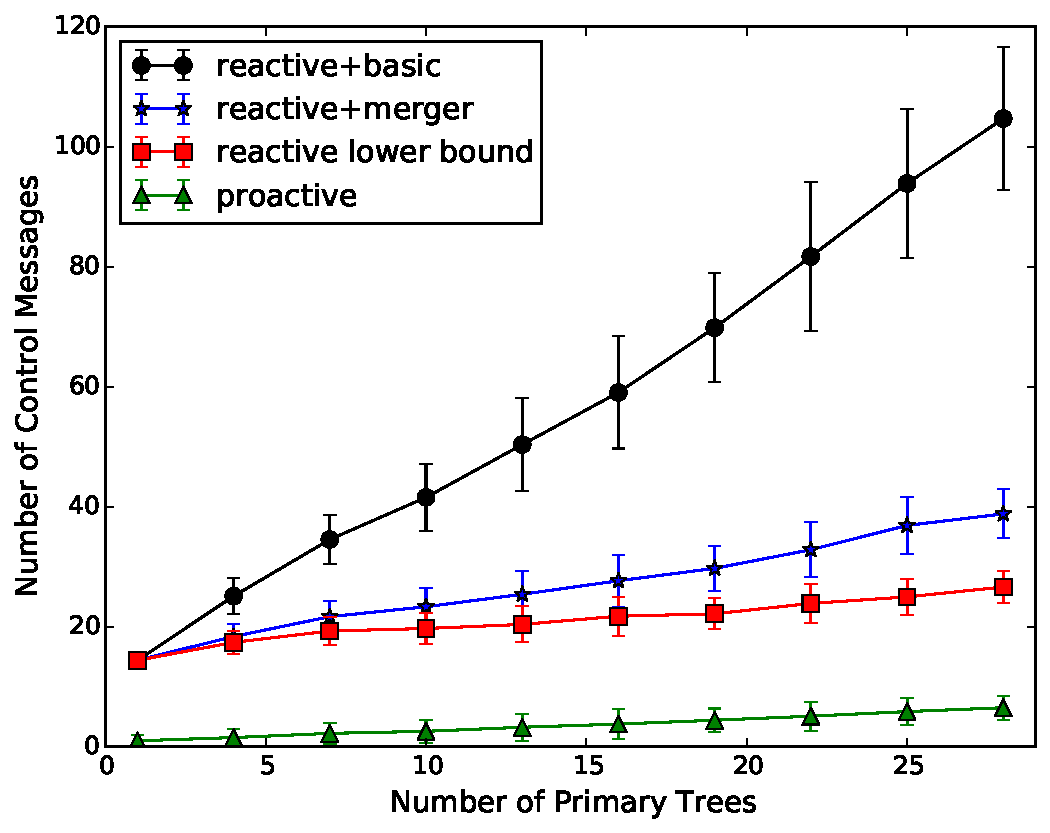
\includegraphics[scale=0.4]{figs/msgs-ieee57.pdf}}
	\subfigure[Total time to install all backup tree flow table entries.]{\label{fig:install-time57}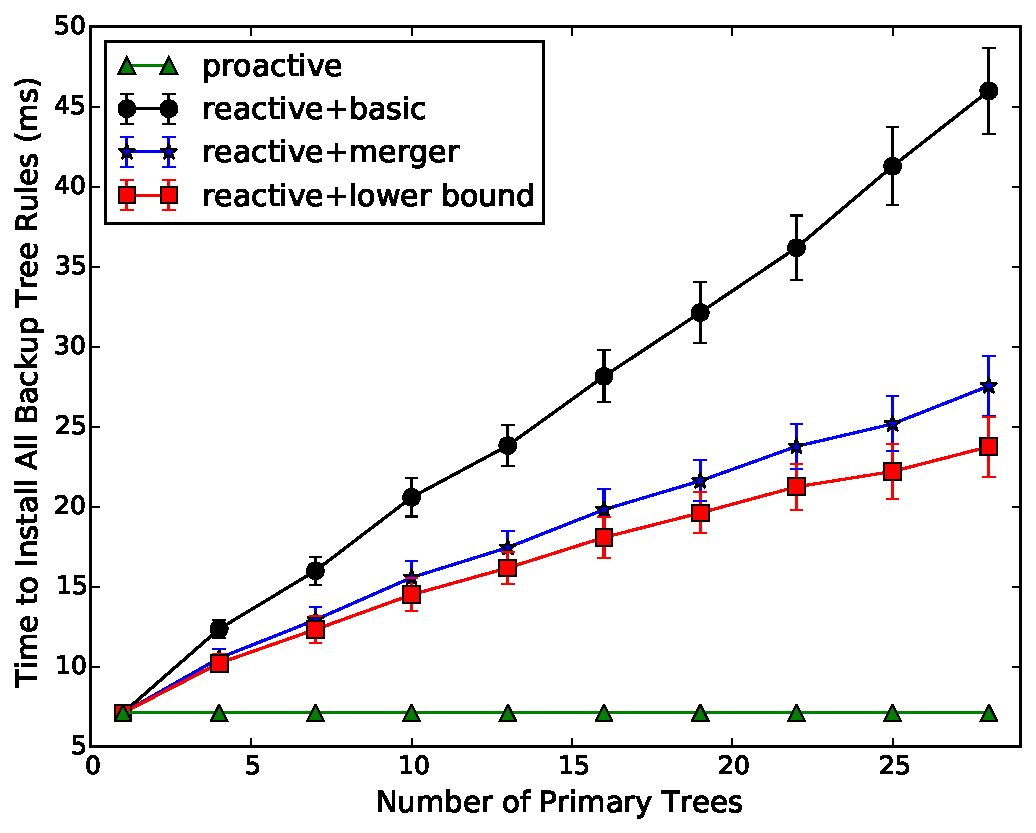
\includegraphics[scale=0.4]{figs/install-time-ieee57.pdf}}
	\subfigure[\pres: mean number of pre-installed rules per switch.]{\label{fig:preinstall57}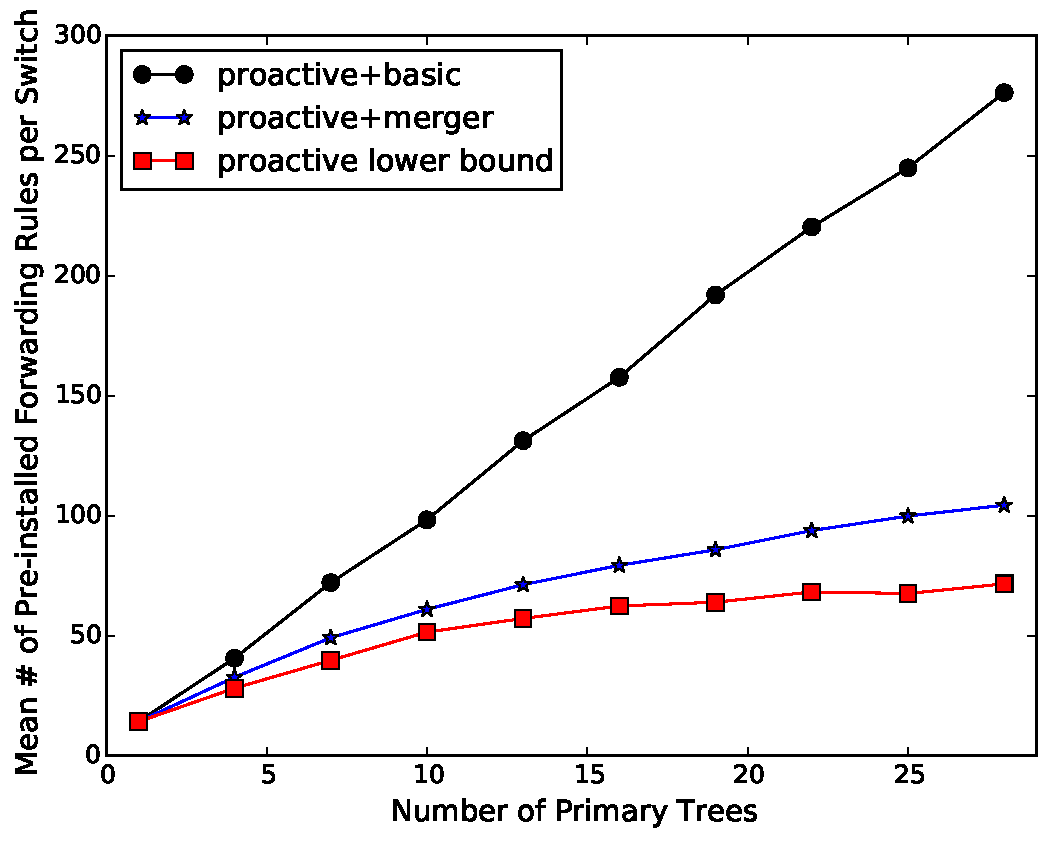
\includegraphics[scale=0.4]{figs/preinstall-ieee57.pdf}}
    %\subfigure[\pres: maximum number of pre-installed rules at a single switch]{\label{fig:preinstall-max57}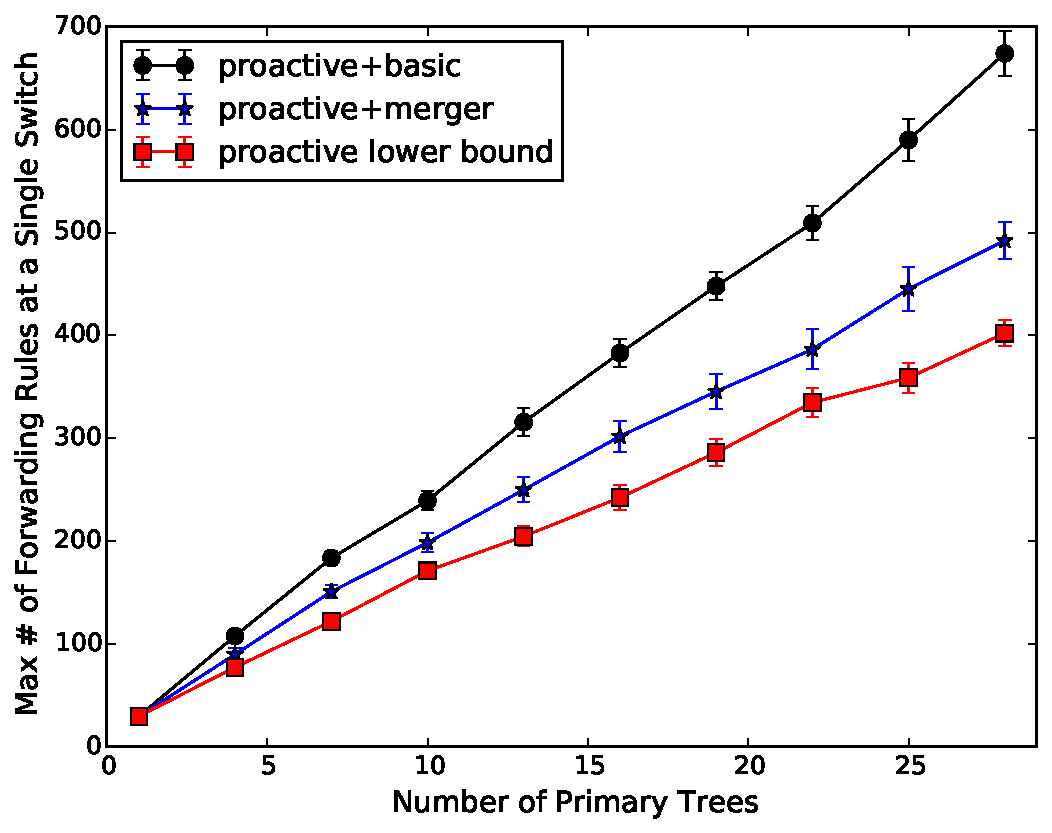
\includegraphics[scale=0.31]{figs/preinstall-max-ieee57.pdf}}
	\subfigure[\posts: number of stale flow table entries resulting from link failure. ]{\label{fig:reactive-garbage57}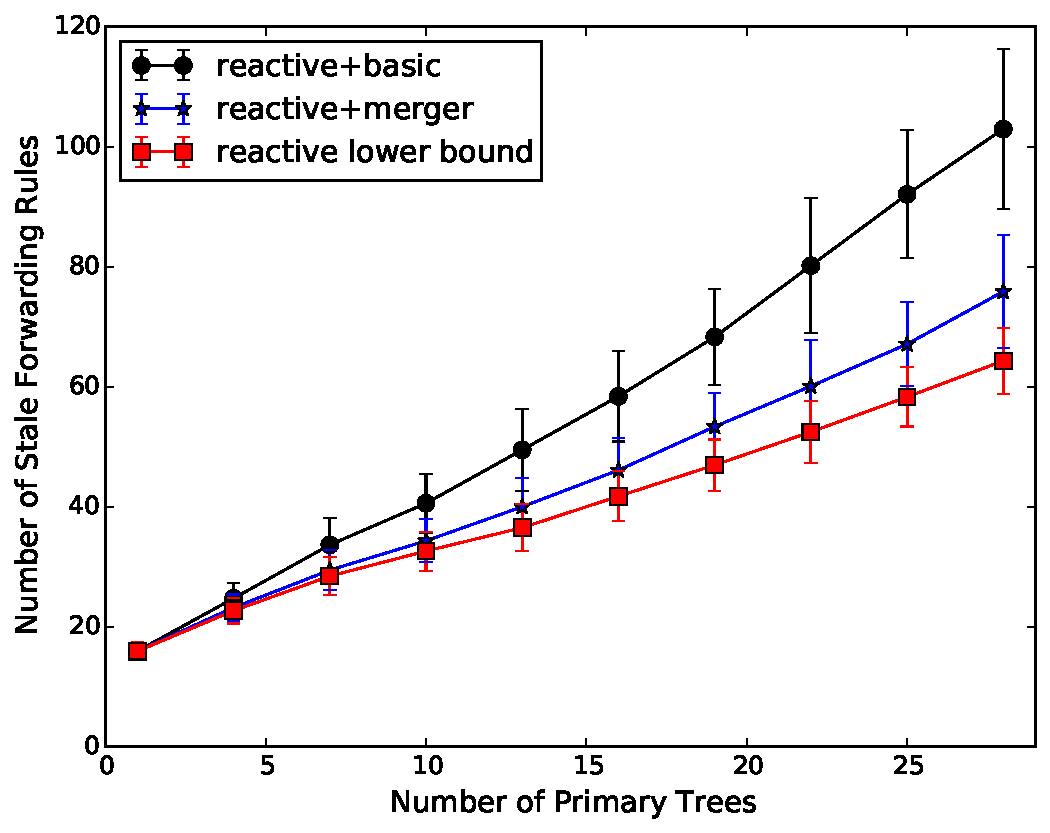
\includegraphics[scale=0.4]{figs/garbage-ieee57.pdf}}
    \subfigure[\pres: number of stale flow table entries resulting from link failure. ]{\label{fig:preinstall-garbage57}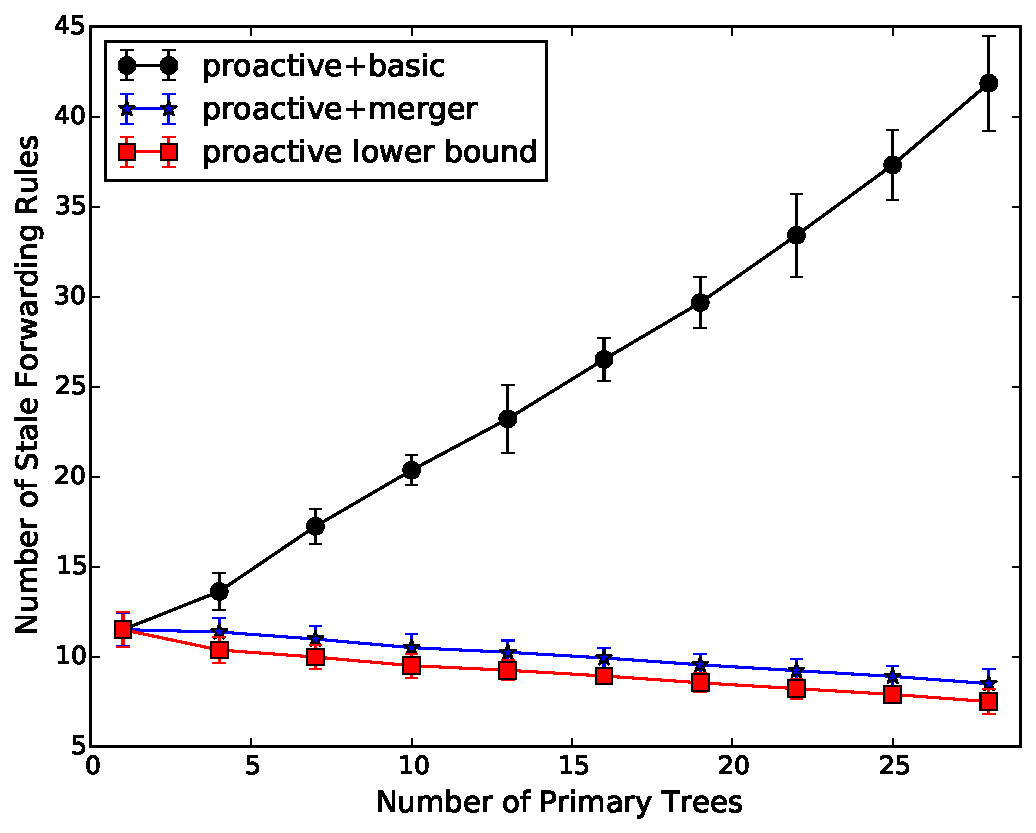
\includegraphics[scale=0.4]{figs/preinstall-garbage-ieee57.pdf}}
  \end{center} 
	\caption{\post and \pre results for a single random link failure of synthetic topologies based on IEEE bus system $57$. 
	Each data point is the mean over $105$ simulation runs and the $95\%$ confidence interval is shown in all plots expect (c).} %\ref{fig:preinstall57}.}
  \label{fig:msgs-preinstall57}
\end{figure*}


